\documentclass[a4paper]{scrreprt}
 
\usepackage[german]{babel}
\usepackage[utf8]{inputenc}
\usepackage[T1]{fontenc}
\usepackage{graphicx}
\graphicspath{ {./Bilder/} }

\usepackage[bookmarks,bookmarksnumbered]{hyperref}
 
\begin{document}
 
\title{Pflichtenheft\\\glqq ClimateSight\grqq}
\author{Leon Fertig (Matrikel-Nummer)\\Matteo Kosina (Matrikel-Nummer) \\Marius Kurth (Matrikel-Nummer)}
\date{\today}
\maketitle


\tableofcontents
 
\chapter{Zielbestimmung}
\section{Muss-Kriterien}
\begin{itemize}
    \item Entwicklung einer Web-Applikation für Desktop-PCs
    \item Start-Seite
    \item Sprache-Einstellungen für Deutsch und Englisch
    \item Weltkarte, die die einzelnen Länder interaktiv mit Informationen verknüpft. Bei Klicken über ein Land erscheinen verschiedene Informationen:
    \begin{itemize}
        \item durchschnittliche Jahrestemperatur (inkl. historische Daten)
        \item Niederschlag pro m$^2$
        \item UV-Einstrahlung
        \item historische Wetterdaten
    \end{itemize}
    \item ausführliche Installationsanleitung
\end{itemize}

\section{Soll-Kriterien}
\begin{itemize}
    \item lokale Nachrichten (mit Fokus auf Klima + Wetter)
    \item Klimafilter (nach Temperatur und/oder Niederschlag)
    \item Anzeige von aktueller Temperatur
\end{itemize}

\section{Kann-Kriterien}
\begin{itemize}
    \item verschiedene Kartenansichten: Satellit, geographisch, Heat-Map
    \item lokale Wetterkarten
\end{itemize}

\section{Abgrenzungskriterien}
\begin{itemize}
    \item kein Einsatz von KI
    \item keine Routenführung
    \item keine mobile Anwendung (nicht für Smartphone oder Tablets optimiert)
\end{itemize}

\chapter{Einsatz}
\section{Anwendungsbereiche}
Klimaüberblick für Interessierte und eine Möglichkeit, sich über die Auswirkungen des Klimawandels und über die Schwankungen im Klima in bestimmten Region zu informieren.

\section{Zielgruppen}
Die Applikation ist auf Leute ausgerichtet, die sich für das Klima und die Folgen des Klimawandels in einem bestimmten Land interessieren.

\section{Betriebsbedingungen}
Dauerhafter Betrieb (24/7), ausgelegt auf einen Nutzer (für Skalierbarkeit wird keine Garantie übernommen), da es nur ein Development-System ist.

\chapter{Umgebung}
\section{Hardware}
Server mit mind. 500 MB Speicher und 1 GB RAM.

\section{Software}
Go 1.21.0

\section{Orgware}
\begin{itemize}
    \item API-Key von OpenStreetMap
    \item API-Key von OpenWeatherMap
\end{itemize}

% \chapter{Funktionalität}
% Funktionalität: Spezifikation der einzelnen Produktfunktionen mit genauer und
% detaillierter Beschreibung.

\chapter{Daten}
Daten von:
\begin{itemize}
    \item OpenStreetMap (\url{https://www.openstreetmap.org})
    \item OpenWeatherMap (\url{https://openweathermap.org})
\end{itemize}

\chapter{Leistungen}
Die Web-Applikation garantiert keine Genauigkeit der Daten, da diese von externen Quellen stammen. Sofern man davon ausgehen kann, dass die bereitgestellten Daten korrekt sind, sind die dargestellten (und evtl. umgerechneten Daten) auch korrekt.

\chapter{Benutzeroberfläche}
Es gibt 3 verschieden Benutzeroberflächen: Die Landing-Page, die Discover-Page und die Analytics-Page. Die Landing-Page gibt einige allgemeine Informationen zum Projekt und beinhaltet einen Button zur Discover-Page; Auf dieser kann der User auf einer Weltkarte nach verschiedenen Ländern filtern, die dann hervorgehoben werden. Klickt der User auf ein bestimmtes Land, wird er zur entsprechenden Analytics-Page dieses Landes weitergeleitet, auf der er verschiedene Informationen und Statistiken zur Wetter- und Klimaentwicklung im jeweiligen Land betrachten kann.
\begin{figure}[ht]
    \centering
    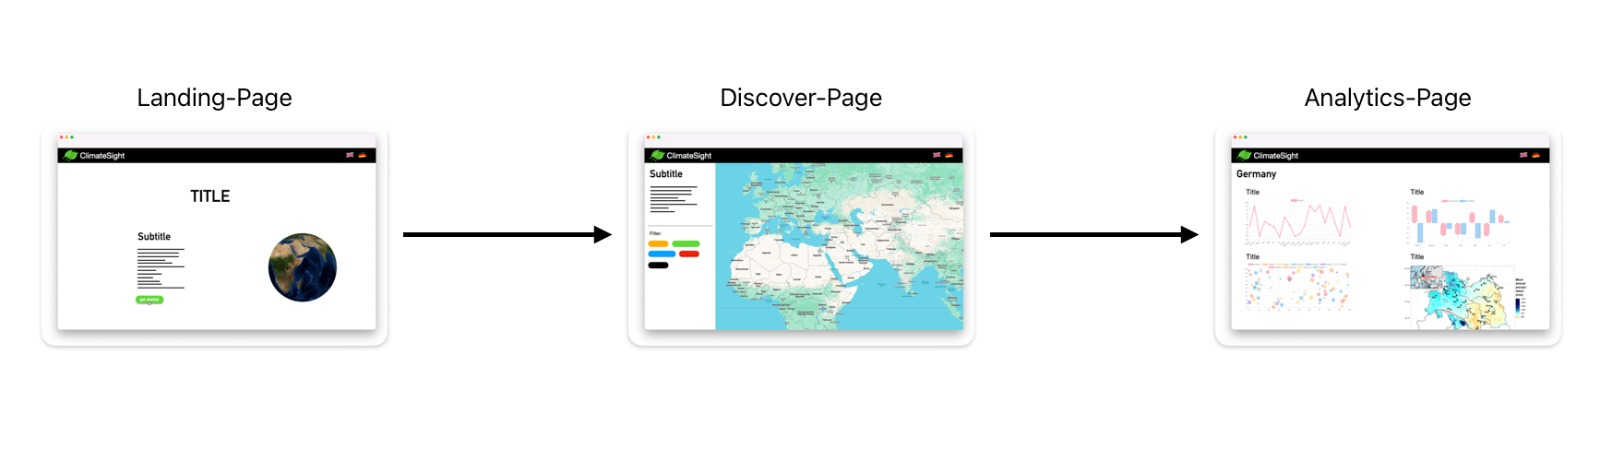
\includegraphics[width=\textwidth]{Uebersicht.jpg}
    \caption{Benutzeroberfläche: Übersicht}
\end{figure}
\begin{figure}[ht]
    \centering
    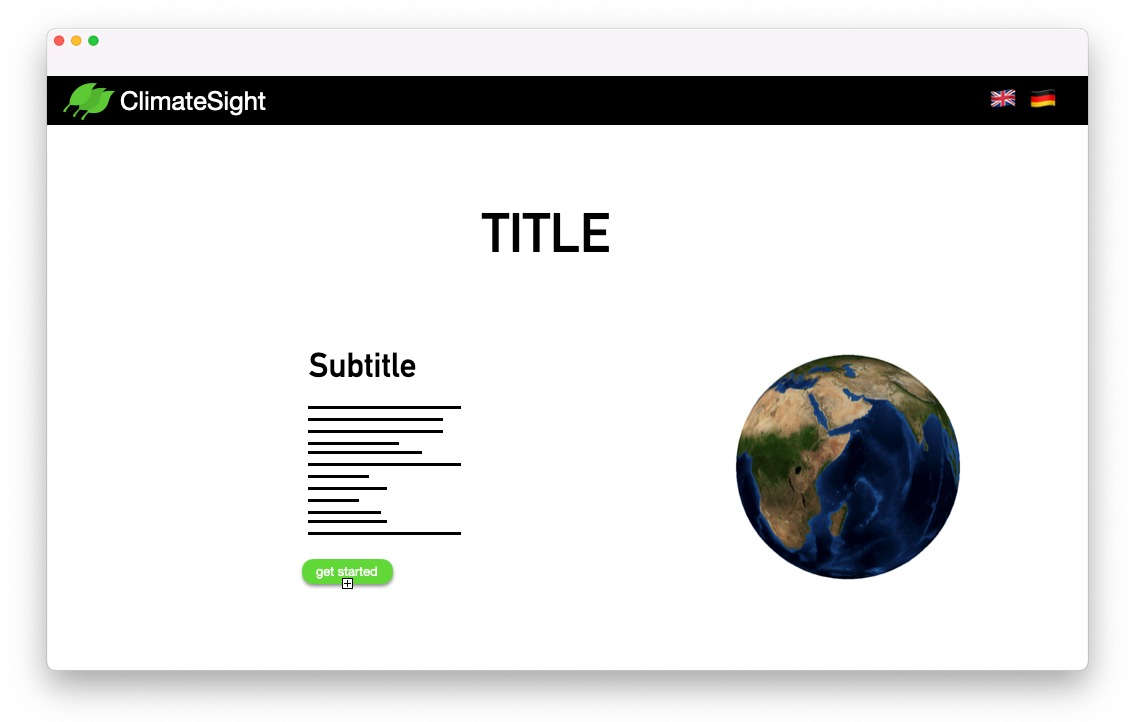
\includegraphics[width=\textwidth]{Landingpage.jpg}
    \caption{Landing-Page}
\end{figure}
\begin{figure}[ht]
    \centering
    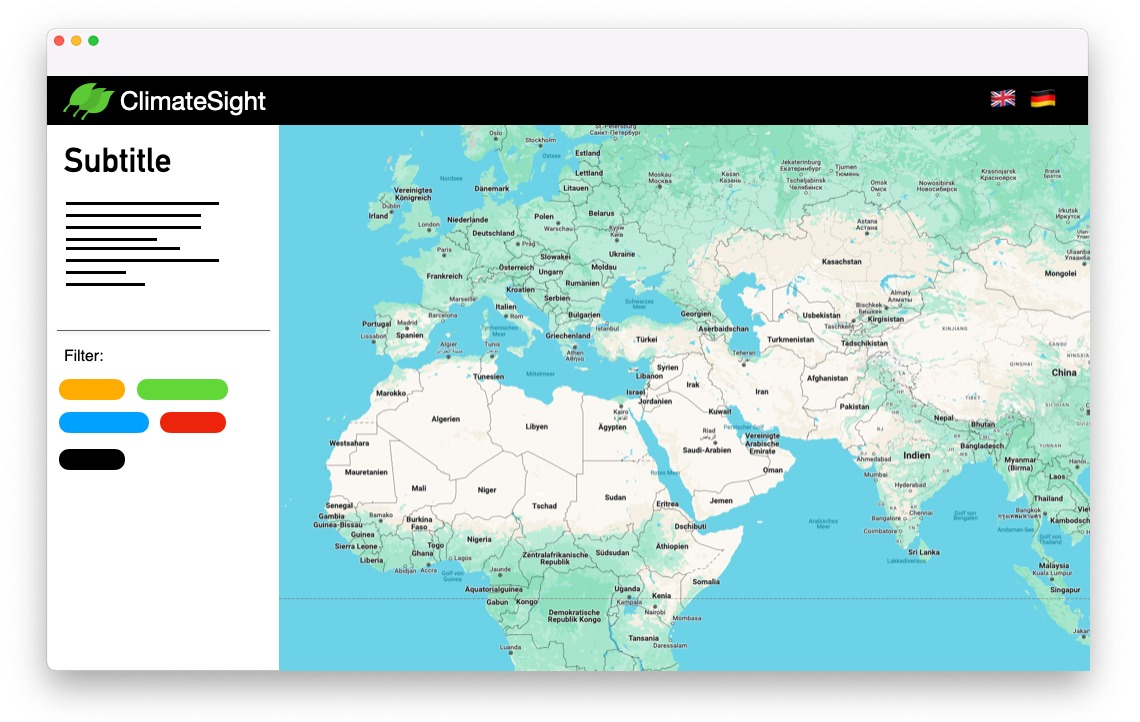
\includegraphics[width=\textwidth]{Kartenansicht.jpg}
    \caption{Discover-Page}
\end{figure}
\begin{figure}[ht]
    \centering
    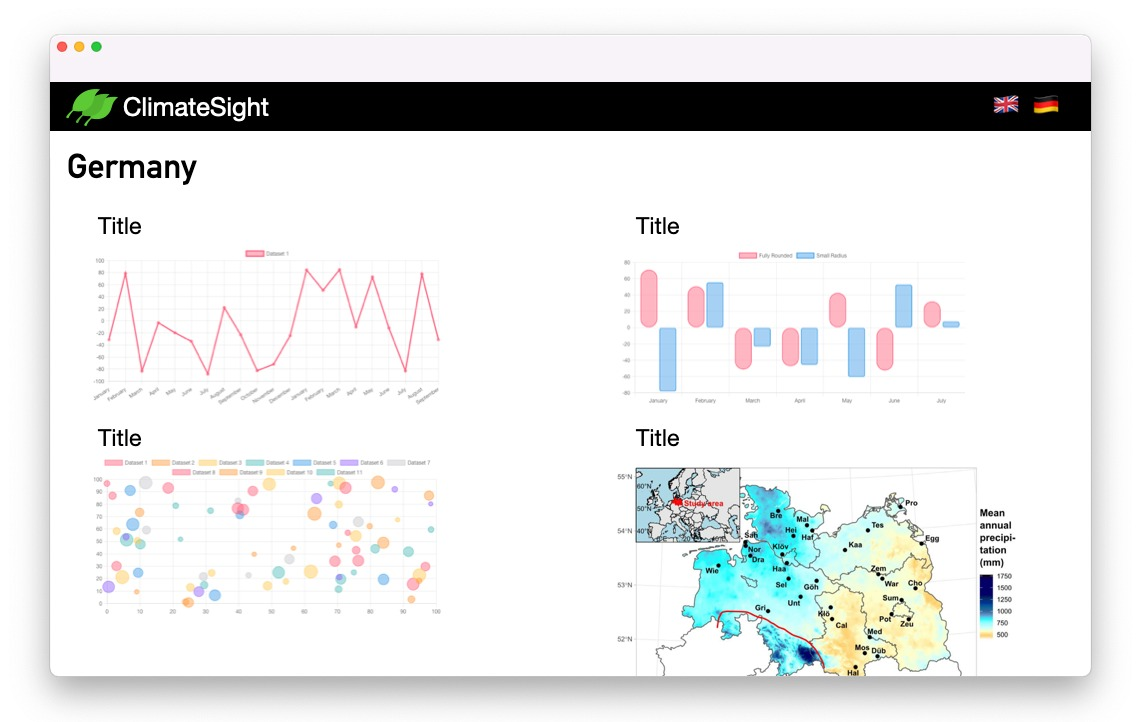
\includegraphics[width=\textwidth]{Laenderansicht.jpg}
    \caption{Analytics-Page}
\end{figure}


% \chapter{Qualitätsziele}
% Qualiätsziele: Allgemeine Ziele sind meistens Änderbarkeit und Wartbarkeit.
% Ziele sollten jedoch grundsätzlich messbar, spezifisch und relevant sein.

\chapter{Ergänzungen}
Es soll OpenStreetMap (\url{https://www.openstreetmap.org}) als Datenquelle für die Geodaten verwendet werden. Für die Wetter- und Klimadaten soll OpenWeatherMap (\url{https://openweathermap.org}) verwendet werden.
Dafür wird jeweils vorausgesetzt, dass der Betreiber der Webseite jeweils einen API-Key (für beide Dienste) besitzt und diese im Backend hinterlegt hat.

\end{document}